\subsection{Description of the given problem}

As already said in the previous section \textit{TrackMe}'s system as the aim to provide different applications to the different actors.
\begin{itemize}
	\item {\textit{D4H and ASOS} app is designed to provide the users with an overview of their health parameters by obtaining them from the device associated to the smartphone that runs it. The device should be able to collect health parameters such as the heart beat and send them to the main app running on the smartphone. If the user has activated the \textit{ASOS} service everytime that a new value is collected the app checks if it is higher or not than the trashold value:
		\begin{itemize}
			\item {if it is upper it is stored in the database;}
			\item {if it is lower the \textit{ASOS} service will be activated and it will contact the outside SOS service in less than 5 seconds from the time the parameters started to be below the threshold. By contacting the SOS service \textit{ASOS} will also give the location of the user who needs medical help.}
		\end{itemize}
		The user can always choose to activate the \textit{ASOS} service by subscribing to it in the designated area. The user can also monitor his/her health parameters by looking the specific app's area.\\
		Anytime a third party will ask to accede to the single user's data the app will send a notification to the specific user to get permission to share his/her data. The user can accept or deny the request.}

	\item{\textit{D4H} app is designed to provide the third parties with the possibility to require single user's or group of users' data.
		If the third party wants to accede to the data of  a specific user it must have his/her secure number or fiscal code. The app is than in charge to ask to the specific user if he/she wants to share his/her data with the third party: if the user accepts, data will be shared; if he/she denies, the third party will receive a notification saying that.\\
		To obtain data of groups of users the third parties must specify some contraints to define the type of data and the type of uses they are interested in; this means that the query can be personalized depending on which type of data the third parties need. The app accepts those requests and sends data if and only if the quantity of users that respect the query's parameters is heigher than 1000; this threshold has been imposed to guarantee users' privacy. in case the number of users is lower than 1000 the third party will receive a notification saying that.\\
		Throught this app a third party can also subscribe for new data, once a request has been accepted the app asks if it would like to receive more data related to the single user or to the group of users of the request.}
		
\end{itemize}

\subsection{World and Machine}
The aim of this subsection is to describe the problem following the World and Machine model. The World domain is the set of all real-life events in which the Machine will be introduced and in which the its actions will be observed. The Machine domain is the set of all phenomena which it can control such as algorithms, devices, inputs from the world.\\
Those two domains are connected via Shared Phenomena which are World's events and Machine's actions which are observable by both domains.

\begin{figure}[h!]
	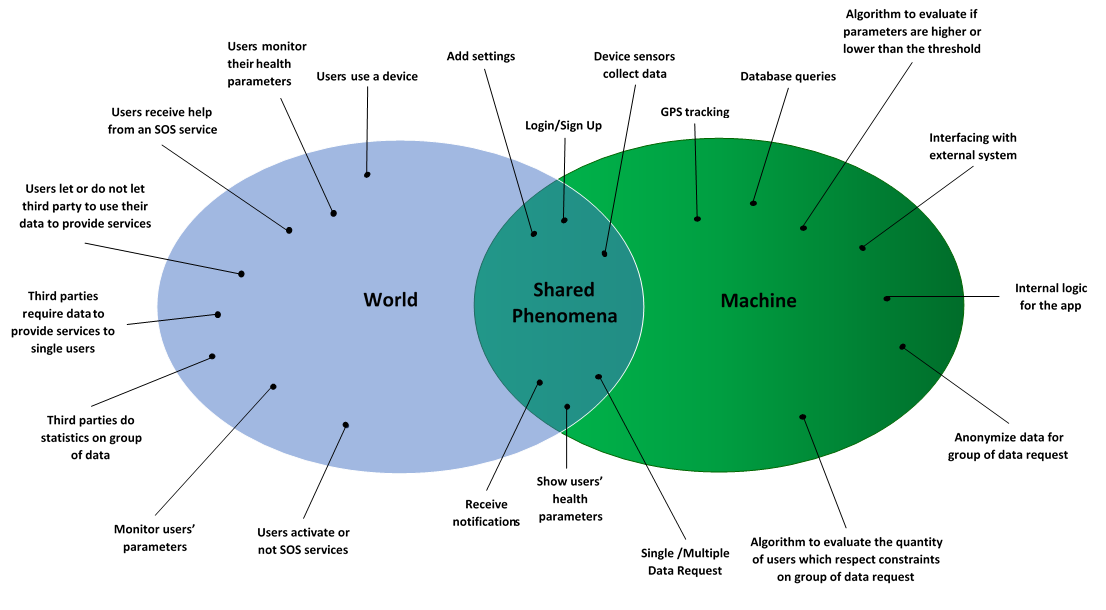
\includegraphics[width=1.00\textwidth]{./pictures/world_machine.png}\par
	\caption{Figure 1: World and Machine diagram}
\end{figure}